\section{Search}
\label{sec:search}

As the search space of possible DSP program is extremely large, our search procedures must be exceptionally efficient. 
As a first foray into DSP-PBE, we restrict ourselves to only synthesizing low-pass and high-pass filters, and global volume adjustment.
These two filters have the key property that they are quasi-commutative -- when the thresholds of these filters do not overlap, applying a low-pass and then a high-pass is the same as applying a high-pass and then a low-pass.
Although our approach has no theoretical basis for being applicable to non-commutative filters (for example, delay lines or ring filters), we do attempt to use our approach on such filters in Sec~\ref{sec:future}.
We leave a more thorough exploration of non-commutative filters to future work.

\subsection{Gradient Descent}

Gradient descent is a technique commonly used in modelling and machine learning.
Given a cost function, which represents the disagreement between a proposed model and the actual data, gradient descent can be used efficiently to minimize the cost and generate the model of best fit.
Gradient descent is only guaranteed to terminate with the globally minimal cost if the cost function being optimized is convex -- this is because gradient descent will ``descend'' along the surface of the cost function, in each step following the steepest gradient.
While we were not able to design our aural distance function from Section~\ref{sec:distance} to be convex, our cost function does demonstrate some properties of convexity that allow gradient descent to produce useful results, even if the result is not guaranteed to be the global minimum.
We will describe here some properties of our distance metric that were helpful in minimizing the cost of the synthesized filter, as well as the shortcomings of our design, and how we try to overcome them by adjusting our implementation of gradient descent.

\begin{figure}[!h]
%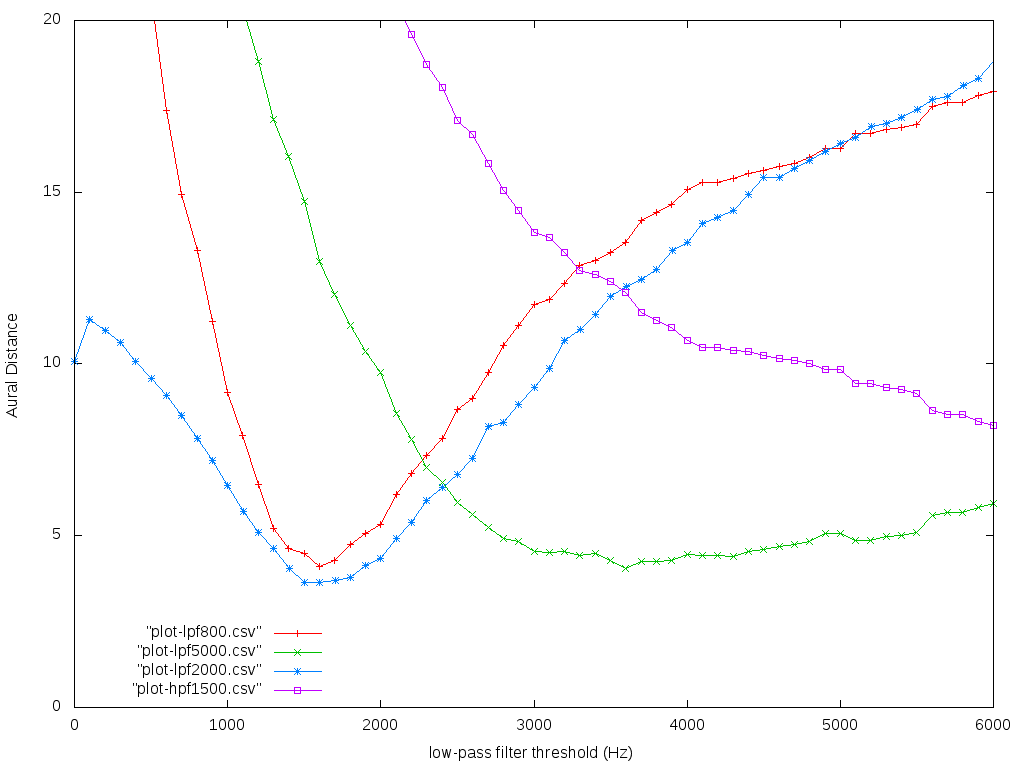
\includegraphics[width=\columnwidth]{figs/distCurves} 
\begin{tikzpicture}[gnuplot]
%% generated with GNUPLOT 5.0p3 (Lua 5.1; terminal rev. 99, script rev. 100)
%% Sun 05 Aug 2018 11:09:39 PM EDT
\path (0.000,0.000) rectangle (8.890,8.890);
\gpcolor{color=gp lt color border}
\gpsetlinetype{gp lt border}
\gpsetlinewidth{1.00}
\draw[gp path] (1.136,0.985)--(1.316,0.985);
\draw[gp path] (8.337,0.985)--(8.157,0.985);
\node[gp node right] at (0.952,0.985) {$0$};
\draw[gp path] (1.136,2.869)--(1.316,2.869);
\draw[gp path] (8.337,2.869)--(8.157,2.869);
\node[gp node right] at (0.952,2.869) {$5$};
\draw[gp path] (1.136,4.753)--(1.316,4.753);
\draw[gp path] (8.337,4.753)--(8.157,4.753);
\node[gp node right] at (0.952,4.753) {$10$};
\draw[gp path] (1.136,6.637)--(1.316,6.637);
\draw[gp path] (8.337,6.637)--(8.157,6.637);
\node[gp node right] at (0.952,6.637) {$15$};
\draw[gp path] (1.136,8.521)--(1.316,8.521);
\draw[gp path] (8.337,8.521)--(8.157,8.521);
\node[gp node right] at (0.952,8.521) {$20$};
\draw[gp path] (1.136,0.985)--(1.136,1.165);
\draw[gp path] (1.136,8.521)--(1.136,8.341);
\node[gp node center] at (1.136,0.677) {$0$};
\draw[gp path] (2.336,0.985)--(2.336,1.165);
\draw[gp path] (2.336,8.521)--(2.336,8.341);
\node[gp node center] at (2.336,0.677) {$1000$};
\draw[gp path] (3.536,0.985)--(3.536,1.165);
\draw[gp path] (3.536,8.521)--(3.536,8.341);
\node[gp node center] at (3.536,0.677) {$2000$};
\draw[gp path] (4.737,0.985)--(4.737,1.165);
\draw[gp path] (4.737,8.521)--(4.737,8.341);
\node[gp node center] at (4.737,0.677) {$3000$};
\draw[gp path] (5.937,0.985)--(5.937,1.165);
\draw[gp path] (5.937,8.521)--(5.937,8.341);
\node[gp node center] at (5.937,0.677) {$4000$};
\draw[gp path] (7.137,0.985)--(7.137,1.165);
\draw[gp path] (7.137,8.521)--(7.137,8.341);
\node[gp node center] at (7.137,0.677) {$5000$};
\draw[gp path] (8.337,0.985)--(8.337,1.165);
\draw[gp path] (8.337,8.521)--(8.337,8.341);
\node[gp node center] at (8.337,0.677) {$6000$};
\draw[gp path] (1.136,8.521)--(1.136,0.985)--(8.337,0.985)--(8.337,8.521)--cycle;
\node[gp node center,rotate=-270] at (0.246,4.753) {Aural Distance};
\node[gp node center] at (4.736,0.215) {low-pass filter threshold (Hz)};
\node[gp node right] at (7.232,1.627) {$\synthFilter = lpf(800)$};
\gpcolor{rgb color={0.580,0.000,0.827}}
\draw[gp path] (7.4,1.627)--(8.2,1.627);
\draw[gp path] (1.766,8.521)--(1.856,7.533)--(1.976,6.610)--(2.096,5.998)--(2.216,5.219)%
  --(2.336,4.443)--(2.456,3.966)--(2.576,3.427)--(2.696,2.946)--(2.816,2.724)--(2.936,2.672)%
  --(3.056,2.528)--(3.176,2.595)--(3.296,2.770)--(3.416,2.897)--(3.536,2.996)--(3.656,3.325)%
  --(3.776,3.551)--(3.896,3.753)--(4.016,3.940)--(4.136,4.257)--(4.256,4.371)--(4.376,4.656)%
  --(4.496,4.955)--(4.616,5.176)--(4.737,5.403)--(4.857,5.460)--(4.977,5.637)--(5.097,5.829)%
  --(5.217,5.890)--(5.337,5.976)--(5.457,6.087)--(5.577,6.323)--(5.697,6.411)--(5.817,6.506)%
  --(5.937,6.665)--(6.057,6.748)--(6.177,6.748)--(6.297,6.783)--(6.417,6.839)--(6.537,6.875)%
  --(6.657,6.918)--(6.777,6.953)--(6.897,7.022)--(7.017,7.118)--(7.137,7.118)--(7.257,7.279)%
  --(7.377,7.279)--(7.497,7.323)--(7.617,7.346)--(7.737,7.383)--(7.857,7.573)--(7.977,7.619)%
  --(8.097,7.619)--(8.217,7.698)--(8.337,7.742);
\gpsetpointsize{4.00}
\gppoint{gp mark 1}{(1.856,7.533)}
\gppoint{gp mark 1}{(1.976,6.610)}
\gppoint{gp mark 1}{(2.096,5.998)}
\gppoint{gp mark 1}{(2.216,5.219)}
\gppoint{gp mark 1}{(2.336,4.443)}
\gppoint{gp mark 1}{(2.456,3.966)}
\gppoint{gp mark 1}{(2.576,3.427)}
\gppoint{gp mark 1}{(2.696,2.946)}
\gppoint{gp mark 1}{(2.816,2.724)}
\gppoint{gp mark 1}{(2.936,2.672)}
\gppoint{gp mark 1}{(3.056,2.528)}
\gppoint{gp mark 1}{(3.176,2.595)}
\gppoint{gp mark 1}{(3.296,2.770)}
\gppoint{gp mark 1}{(3.416,2.897)}
\gppoint{gp mark 1}{(3.536,2.996)}
\gppoint{gp mark 1}{(3.656,3.325)}
\gppoint{gp mark 1}{(3.776,3.551)}
\gppoint{gp mark 1}{(3.896,3.753)}
\gppoint{gp mark 1}{(4.016,3.940)}
\gppoint{gp mark 1}{(4.136,4.257)}
\gppoint{gp mark 1}{(4.256,4.371)}
\gppoint{gp mark 1}{(4.376,4.656)}
\gppoint{gp mark 1}{(4.496,4.955)}
\gppoint{gp mark 1}{(4.616,5.176)}
\gppoint{gp mark 1}{(4.737,5.403)}
\gppoint{gp mark 1}{(4.857,5.460)}
\gppoint{gp mark 1}{(4.977,5.637)}
\gppoint{gp mark 1}{(5.097,5.829)}
\gppoint{gp mark 1}{(5.217,5.890)}
\gppoint{gp mark 1}{(5.337,5.976)}
\gppoint{gp mark 1}{(5.457,6.087)}
\gppoint{gp mark 1}{(5.577,6.323)}
\gppoint{gp mark 1}{(5.697,6.411)}
\gppoint{gp mark 1}{(5.817,6.506)}
\gppoint{gp mark 1}{(5.937,6.665)}
\gppoint{gp mark 1}{(6.057,6.748)}
\gppoint{gp mark 1}{(6.177,6.748)}
\gppoint{gp mark 1}{(6.297,6.783)}
\gppoint{gp mark 1}{(6.417,6.839)}
\gppoint{gp mark 1}{(6.537,6.875)}
\gppoint{gp mark 1}{(6.657,6.918)}
\gppoint{gp mark 1}{(6.777,6.953)}
\gppoint{gp mark 1}{(6.897,7.022)}
\gppoint{gp mark 1}{(7.017,7.118)}
\gppoint{gp mark 1}{(7.137,7.118)}
\gppoint{gp mark 1}{(7.257,7.279)}
\gppoint{gp mark 1}{(7.377,7.279)}
\gppoint{gp mark 1}{(7.497,7.323)}
\gppoint{gp mark 1}{(7.617,7.346)}
\gppoint{gp mark 1}{(7.737,7.383)}
\gppoint{gp mark 1}{(7.857,7.573)}
\gppoint{gp mark 1}{(7.977,7.619)}
\gppoint{gp mark 1}{(8.097,7.619)}
\gppoint{gp mark 1}{(8.217,7.698)}
\gppoint{gp mark 1}{(8.337,7.742)}
\gppoint{gp mark 1}{(7.8,1.62)}
\gpcolor{color=gp lt color border}
\node[gp node right] at (7.232,1.319) {$\synthFilter = lpf(5000)$};
\gpcolor{rgb color={0.000,0.620,0.451}}
\draw[gp path] (7.4,1.319)--(8.2,1.319);
\draw[gp path] (2.485,8.521)--(2.575,8.071)--(2.696,7.440)--(2.816,7.024)--(2.936,6.541)%
  --(3.056,5.883)--(3.176,5.510)--(3.296,5.173)--(3.416,4.893)--(3.536,4.656)--(3.656,4.208)%
  --(3.776,3.926)--(3.896,3.619)--(4.016,3.458)--(4.136,3.239)--(4.256,3.100)--(4.376,2.964)%
  --(4.496,2.841)--(4.616,2.810)--(4.737,2.693)--(4.857,2.688)--(4.977,2.693)--(5.097,2.657)%
  --(5.217,2.677)--(5.337,2.595)--(5.457,2.510)--(5.577,2.583)--(5.697,2.583)--(5.817,2.601)%
  --(5.937,2.658)--(6.057,2.654)--(6.177,2.654)--(6.297,2.644)--(6.417,2.700)--(6.537,2.713)%
  --(6.657,2.757)--(6.777,2.772)--(6.897,2.806)--(7.017,2.888)--(7.137,2.888)--(7.257,2.821)%
  --(7.377,2.821)--(7.497,2.864)--(7.617,2.870)--(7.737,2.899)--(7.857,3.089)--(7.977,3.119)%
  --(8.097,3.119)--(8.217,3.180)--(8.337,3.224);
\gppoint{gp mark 2}{(2.575,8.071)}
\gppoint{gp mark 2}{(2.696,7.440)}
\gppoint{gp mark 2}{(2.816,7.024)}
\gppoint{gp mark 2}{(2.936,6.541)}
\gppoint{gp mark 2}{(3.056,5.883)}
\gppoint{gp mark 2}{(3.176,5.510)}
\gppoint{gp mark 2}{(3.296,5.173)}
\gppoint{gp mark 2}{(3.416,4.893)}
\gppoint{gp mark 2}{(3.536,4.656)}
\gppoint{gp mark 2}{(3.656,4.208)}
\gppoint{gp mark 2}{(3.776,3.926)}
\gppoint{gp mark 2}{(3.896,3.619)}
\gppoint{gp mark 2}{(4.016,3.458)}
\gppoint{gp mark 2}{(4.136,3.239)}
\gppoint{gp mark 2}{(4.256,3.100)}
\gppoint{gp mark 2}{(4.376,2.964)}
\gppoint{gp mark 2}{(4.496,2.841)}
\gppoint{gp mark 2}{(4.616,2.810)}
\gppoint{gp mark 2}{(4.737,2.693)}
\gppoint{gp mark 2}{(4.857,2.688)}
\gppoint{gp mark 2}{(4.977,2.693)}
\gppoint{gp mark 2}{(5.097,2.657)}
\gppoint{gp mark 2}{(5.217,2.677)}
\gppoint{gp mark 2}{(5.337,2.595)}
\gppoint{gp mark 2}{(5.457,2.510)}
\gppoint{gp mark 2}{(5.577,2.583)}
\gppoint{gp mark 2}{(5.697,2.583)}
\gppoint{gp mark 2}{(5.817,2.601)}
\gppoint{gp mark 2}{(5.937,2.658)}
\gppoint{gp mark 2}{(6.057,2.654)}
\gppoint{gp mark 2}{(6.177,2.654)}
\gppoint{gp mark 2}{(6.297,2.644)}
\gppoint{gp mark 2}{(6.417,2.700)}
\gppoint{gp mark 2}{(6.537,2.713)}
\gppoint{gp mark 2}{(6.657,2.757)}
\gppoint{gp mark 2}{(6.777,2.772)}
\gppoint{gp mark 2}{(6.897,2.806)}
\gppoint{gp mark 2}{(7.017,2.888)}
\gppoint{gp mark 2}{(7.137,2.888)}
\gppoint{gp mark 2}{(7.257,2.821)}
\gppoint{gp mark 2}{(7.377,2.821)}
\gppoint{gp mark 2}{(7.497,2.864)}
\gppoint{gp mark 2}{(7.617,2.870)}
\gppoint{gp mark 2}{(7.737,2.899)}
\gppoint{gp mark 2}{(7.857,3.089)}
\gppoint{gp mark 2}{(7.977,3.119)}
\gppoint{gp mark 2}{(8.097,3.119)}
\gppoint{gp mark 2}{(8.217,3.180)}
\gppoint{gp mark 2}{(8.337,3.224)}
\gppoint{gp mark 2}{(7.8,1.309)}
\gpcolor{color=gp lt color border}
\node[gp node right] at (3.832,1.627) {$\synthFilter = lpf(2000)$};
\gpcolor{rgb color={0.337,0.706,0.914}}
\draw[gp path] (4.016,1.627)--(4.732,1.627);
\draw[gp path] (1.136,4.779)--(1.256,5.242)--(1.376,5.125)--(1.497,4.985)--(1.617,4.777)%
  --(1.737,4.589)--(1.857,4.409)--(1.977,4.185)--(2.097,3.932)--(2.217,3.691)--(2.337,3.424)%
  --(2.457,3.131)--(2.577,2.901)--(2.697,2.730)--(2.817,2.513)--(2.937,2.359)--(3.057,2.354)%
  --(3.177,2.374)--(3.298,2.413)--(3.418,2.542)--(3.538,2.621)--(3.658,2.838)--(3.778,3.019)%
  --(3.898,3.251)--(4.018,3.402)--(4.138,3.544)--(4.258,3.720)--(4.378,4.071)--(4.498,4.109)%
  --(4.618,4.312)--(4.738,4.495)--(4.858,4.707)--(4.978,5.015)--(5.098,5.129)--(5.218,5.291)%
  --(5.338,5.492)--(5.458,5.602)--(5.578,5.684)--(5.698,5.794)--(5.818,6.003)--(5.938,6.090)%
  --(6.058,6.290)--(6.178,6.365)--(6.298,6.432)--(6.418,6.609)--(6.538,6.794)--(6.658,6.794)%
  --(6.778,6.898)--(6.898,6.990)--(7.018,7.083)--(7.138,7.168)--(7.258,7.243)--(7.378,7.358)%
  --(7.498,7.391)--(7.618,7.462)--(7.738,7.539)--(7.858,7.652)--(7.978,7.688)--(8.098,7.811)%
  --(8.218,7.889)--(8.337,8.076);
\gppoint{gp mark 3}{(1.136,4.779)}
\gppoint{gp mark 3}{(1.256,5.242)}
\gppoint{gp mark 3}{(1.376,5.125)}
\gppoint{gp mark 3}{(1.497,4.985)}
\gppoint{gp mark 3}{(1.617,4.777)}
\gppoint{gp mark 3}{(1.737,4.589)}
\gppoint{gp mark 3}{(1.857,4.409)}
\gppoint{gp mark 3}{(1.977,4.185)}
\gppoint{gp mark 3}{(2.097,3.932)}
\gppoint{gp mark 3}{(2.217,3.691)}
\gppoint{gp mark 3}{(2.337,3.424)}
\gppoint{gp mark 3}{(2.457,3.131)}
\gppoint{gp mark 3}{(2.577,2.901)}
\gppoint{gp mark 3}{(2.697,2.730)}
\gppoint{gp mark 3}{(2.817,2.513)}
\gppoint{gp mark 3}{(2.937,2.359)}
\gppoint{gp mark 3}{(3.057,2.354)}
\gppoint{gp mark 3}{(3.177,2.374)}
\gppoint{gp mark 3}{(3.298,2.413)}
\gppoint{gp mark 3}{(3.418,2.542)}
\gppoint{gp mark 3}{(3.538,2.621)}
\gppoint{gp mark 3}{(3.658,2.838)}
\gppoint{gp mark 3}{(3.778,3.019)}
\gppoint{gp mark 3}{(3.898,3.251)}
\gppoint{gp mark 3}{(4.018,3.402)}
\gppoint{gp mark 3}{(4.138,3.544)}
\gppoint{gp mark 3}{(4.258,3.720)}
\gppoint{gp mark 3}{(4.378,4.071)}
\gppoint{gp mark 3}{(4.498,4.109)}
\gppoint{gp mark 3}{(4.618,4.312)}
\gppoint{gp mark 3}{(4.738,4.495)}
\gppoint{gp mark 3}{(4.858,4.707)}
\gppoint{gp mark 3}{(4.978,5.015)}
\gppoint{gp mark 3}{(5.098,5.129)}
\gppoint{gp mark 3}{(5.218,5.291)}
\gppoint{gp mark 3}{(5.338,5.492)}
\gppoint{gp mark 3}{(5.458,5.602)}
\gppoint{gp mark 3}{(5.578,5.684)}
\gppoint{gp mark 3}{(5.698,5.794)}
\gppoint{gp mark 3}{(5.818,6.003)}
\gppoint{gp mark 3}{(5.938,6.090)}
\gppoint{gp mark 3}{(6.058,6.290)}
\gppoint{gp mark 3}{(6.178,6.365)}
\gppoint{gp mark 3}{(6.298,6.432)}
\gppoint{gp mark 3}{(6.418,6.609)}
\gppoint{gp mark 3}{(6.538,6.794)}
\gppoint{gp mark 3}{(6.658,6.794)}
\gppoint{gp mark 3}{(6.778,6.898)}
\gppoint{gp mark 3}{(6.898,6.990)}
\gppoint{gp mark 3}{(7.018,7.083)}
\gppoint{gp mark 3}{(7.138,7.168)}
\gppoint{gp mark 3}{(7.258,7.243)}
\gppoint{gp mark 3}{(7.378,7.358)}
\gppoint{gp mark 3}{(7.498,7.391)}
\gppoint{gp mark 3}{(7.618,7.462)}
\gppoint{gp mark 3}{(7.738,7.539)}
\gppoint{gp mark 3}{(7.858,7.652)}
\gppoint{gp mark 3}{(7.978,7.688)}
\gppoint{gp mark 3}{(8.098,7.811)}
\gppoint{gp mark 3}{(8.218,7.889)}
\gppoint{gp mark 3}{(4.374,1.627)}
\gpcolor{color=gp lt color border}
\node[gp node right] at (3.832,1.319) {$\synthFilter = hpf(1500)$};
\gpcolor{rgb color={0.902,0.624,0.000}}
\draw[gp path] (4.016,1.319)--(4.732,1.319);
\draw[gp path] (3.721,8.521)--(3.776,8.373)--(3.896,8.034)--(4.016,7.788)--(4.136,7.425)%
  --(4.256,7.265)--(4.376,6.956)--(4.496,6.652)--(4.616,6.435)--(4.737,6.199)--(4.857,6.144)%
  --(4.977,5.971)--(5.097,5.778)--(5.217,5.739)--(5.337,5.653)--(5.457,5.538)--(5.577,5.320)%
  --(5.697,5.232)--(5.817,5.155)--(5.937,5.014)--(6.057,4.937)--(6.177,4.937)--(6.297,4.902)%
  --(6.417,4.886)--(6.537,4.851)--(6.657,4.809)--(6.777,4.792)--(6.897,4.755)--(7.017,4.693)%
  --(7.137,4.693)--(7.257,4.535)--(7.377,4.535)--(7.497,4.491)--(7.617,4.468)--(7.737,4.433)%
  --(7.857,4.248)--(7.977,4.202)--(8.097,4.202)--(8.217,4.127)--(8.337,4.084);
\gppoint{gp mark 4}{(3.776,8.373)}
\gppoint{gp mark 4}{(3.896,8.034)}
\gppoint{gp mark 4}{(4.016,7.788)}
\gppoint{gp mark 4}{(4.136,7.425)}
\gppoint{gp mark 4}{(4.256,7.265)}
\gppoint{gp mark 4}{(4.376,6.956)}
\gppoint{gp mark 4}{(4.496,6.652)}
\gppoint{gp mark 4}{(4.616,6.435)}
\gppoint{gp mark 4}{(4.737,6.199)}
\gppoint{gp mark 4}{(4.857,6.144)}
\gppoint{gp mark 4}{(4.977,5.971)}
\gppoint{gp mark 4}{(5.097,5.778)}
\gppoint{gp mark 4}{(5.217,5.739)}
\gppoint{gp mark 4}{(5.337,5.653)}
\gppoint{gp mark 4}{(5.457,5.538)}
\gppoint{gp mark 4}{(5.577,5.320)}
\gppoint{gp mark 4}{(5.697,5.232)}
\gppoint{gp mark 4}{(5.817,5.155)}
\gppoint{gp mark 4}{(5.937,5.014)}
\gppoint{gp mark 4}{(6.057,4.937)}
\gppoint{gp mark 4}{(6.177,4.937)}
\gppoint{gp mark 4}{(6.297,4.902)}
\gppoint{gp mark 4}{(6.417,4.886)}
\gppoint{gp mark 4}{(6.537,4.851)}
\gppoint{gp mark 4}{(6.657,4.809)}
\gppoint{gp mark 4}{(6.777,4.792)}
\gppoint{gp mark 4}{(6.897,4.755)}
\gppoint{gp mark 4}{(7.017,4.693)}
\gppoint{gp mark 4}{(7.137,4.693)}
\gppoint{gp mark 4}{(7.257,4.535)}
\gppoint{gp mark 4}{(7.377,4.535)}
\gppoint{gp mark 4}{(7.497,4.491)}
\gppoint{gp mark 4}{(7.617,4.468)}
\gppoint{gp mark 4}{(7.737,4.433)}
\gppoint{gp mark 4}{(7.857,4.248)}
\gppoint{gp mark 4}{(7.977,4.202)}
\gppoint{gp mark 4}{(8.097,4.202)}
\gppoint{gp mark 4}{(8.217,4.127)}
\gppoint{gp mark 4}{(8.337,4.084)}
\gppoint{gp mark 4}{(4.374,1.319)}
\gpcolor{color=gp lt color border}
\draw[gp path] (1.136,8.521)--(1.136,0.985)--(8.337,0.985)--(8.337,8.521)--cycle;
%% coordinates of the plot area
\gpdefrectangularnode{gp plot 1}{\pgfpoint{1.136cm}{0.985cm}}{\pgfpoint{8.337cm}{8.521cm}}
\end{tikzpicture}
%% gnuplot variables

\caption{The distance curves showing the convex-like shape of the aural distance function. Each curve is the distance between an input file, and a filter applied to that file - $dist(I, \synthFilter(I))$.}
\label{fig:distCurves}
\end{figure}

In order to visualize the rough shape of our distance metric, we plot the distance between pairs of examples, and various possible DSP filters in Figure~\ref{fig:distCurves}.
Here we only visualize the distance curves in the dimension of the low-pass filter.
Notice that the curves exhibit a clear ``saddle'', which represents the minimum cost.
In the ideal case, gradient descent will find these points.
Note that we do not have these graphs available during synthesis -- producing the entire graph as in Figure~\ref{fig:distCurves} is prohibitively expensive.

In Figure~\ref{fig:distCurves}, the last curve we plot is the distance between \texttt{cartoon-spring.wav} and \texttt{cartoon-spring-hpf1500.wav}, the same file with a high pass filter applied with a threshold of 1500 Hz.
Notice that as the threshold of the low-pass filter applied to the input example (\texttt{cartoon-spring.wav} increases, the distance to the output example decreases. 
This is because as a low-pass filter's threshold increases, it allows more and more frequencies to pass into the output -- thereby having less of an effect.
Whereas in the case of the \texttt{cartoon-spring-hpf1500.wav}, the true filter is a high-pass filter, so the less we apply a low-pass filter, the closer we get to the correct filter.

\begin{figure}
%\includegraphics[width=\columnwidth]{figs/distCurveZoom} 
\begin{tikzpicture}[gnuplot]
%% generated with GNUPLOT 5.0p3 (Lua 5.1; terminal rev. 99, script rev. 100)
%% Sun 05 Aug 2018 11:05:50 PM EDT
\path (0.000,0.000) rectangle (8.890,8.890);
\gpcolor{color=gp lt color border}
\gpsetlinetype{gp lt border}
\gpsetlinewidth{1.00}
\draw[gp path] (1.320,0.985)--(1.500,0.985);
\draw[gp path] (8.337,0.985)--(8.157,0.985);
\node[gp node right] at (1.136,0.985) {$4$};
\draw[gp path] (1.320,1.927)--(1.500,1.927);
\draw[gp path] (8.337,1.927)--(8.157,1.927);
\node[gp node right] at (1.136,1.927) {$4.5$};
\draw[gp path] (1.320,2.869)--(1.500,2.869);
\draw[gp path] (8.337,2.869)--(8.157,2.869);
\node[gp node right] at (1.136,2.869) {$5$};
\draw[gp path] (1.320,3.811)--(1.500,3.811);
\draw[gp path] (8.337,3.811)--(8.157,3.811);
\node[gp node right] at (1.136,3.811) {$5.5$};
\draw[gp path] (1.320,4.753)--(1.500,4.753);
\draw[gp path] (8.337,4.753)--(8.157,4.753);
\node[gp node right] at (1.136,4.753) {$6$};
\draw[gp path] (1.320,5.695)--(1.500,5.695);
\draw[gp path] (8.337,5.695)--(8.157,5.695);
\node[gp node right] at (1.136,5.695) {$6.5$};
\draw[gp path] (1.320,6.637)--(1.500,6.637);
\draw[gp path] (8.337,6.637)--(8.157,6.637);
\node[gp node right] at (1.136,6.637) {$7$};
\draw[gp path] (1.320,7.579)--(1.500,7.579);
\draw[gp path] (8.337,7.579)--(8.157,7.579);
\node[gp node right] at (1.136,7.579) {$7.5$};
\draw[gp path] (1.320,8.521)--(1.500,8.521);
\draw[gp path] (8.337,8.521)--(8.157,8.521);
\node[gp node right] at (1.136,8.521) {$8$};
\draw[gp path] (1.320,0.985)--(1.320,1.165);
\draw[gp path] (1.320,8.521)--(1.320,8.341);
\node[gp node center] at (1.320,0.677) {$1050$};
\draw[gp path] (2.100,0.985)--(2.100,1.165);
\draw[gp path] (2.100,8.521)--(2.100,8.341);
\node[gp node center] at (2.100,0.677) {$1100$};
\draw[gp path] (2.879,0.985)--(2.879,1.165);
\draw[gp path] (2.879,8.521)--(2.879,8.341);
\node[gp node center] at (2.879,0.677) {$1150$};
\draw[gp path] (3.659,0.985)--(3.659,1.165);
\draw[gp path] (3.659,8.521)--(3.659,8.341);
\node[gp node center] at (3.659,0.677) {$1200$};
\draw[gp path] (4.439,0.985)--(4.439,1.165);
\draw[gp path] (4.439,8.521)--(4.439,8.341);
\node[gp node center] at (4.439,0.677) {$1250$};
\draw[gp path] (5.218,0.985)--(5.218,1.165);
\draw[gp path] (5.218,8.521)--(5.218,8.341);
\node[gp node center] at (5.218,0.677) {$1300$};
\draw[gp path] (5.998,0.985)--(5.998,1.165);
\draw[gp path] (5.998,8.521)--(5.998,8.341);
\node[gp node center] at (5.998,0.677) {$1350$};
\draw[gp path] (6.778,0.985)--(6.778,1.165);
\draw[gp path] (6.778,8.521)--(6.778,8.341);
\node[gp node center] at (6.778,0.677) {$1400$};
\draw[gp path] (7.557,0.985)--(7.557,1.165);
\draw[gp path] (7.557,8.521)--(7.557,8.341);
\node[gp node center] at (7.557,0.677) {$1450$};
\draw[gp path] (8.337,0.985)--(8.337,1.165);
\draw[gp path] (8.337,8.521)--(8.337,8.341);
\node[gp node center] at (8.337,0.677) {$1500$};
\draw[gp path] (1.320,8.521)--(1.320,0.985)--(8.337,0.985)--(8.337,8.521)--cycle;
\node[gp node center,rotate=-270] at (0.246,4.753) {Aural Distance};
\node[gp node center] at (4.828,0.215) {low-pass filter threshold (Hz)};
\node[gp node right] at (4.632,1.319) {$\synthFilter = lpf(800)$};
\gpcolor{rgb color={0.580,0.000,0.827}}
\draw[gp path] (4.816,1.319)--(5.732,1.319);
\draw[gp path] (2.084,8.354)--(2.178,8.240)--(2.256,8.228)--(2.334,8.092)--(2.412,8.047)%
  --(2.490,7.691)--(2.567,7.545)--(2.645,7.380)--(2.723,7.350)--(2.801,6.827)--(2.879,6.827)%
  --(2.957,6.620)--(3.035,6.620)--(3.113,6.442)--(3.191,6.245)--(3.269,6.245)--(3.347,6.157)%
  --(3.425,5.660)--(3.503,5.660)--(3.581,5.660)--(3.659,5.660)--(3.737,5.605)--(3.815,5.470)%
  --(3.893,5.274)--(3.971,4.925)--(4.049,4.726)--(4.127,4.445)--(4.205,4.445)--(4.283,4.318)%
  --(4.361,4.115)--(4.439,3.914)--(4.517,3.914)--(4.595,3.895)--(4.673,3.736)--(4.751,3.753)%
  --(4.829,3.753)--(4.906,3.753)--(4.984,3.758)--(5.062,3.558)--(5.140,3.320)--(5.218,3.253)%
  --(5.296,3.253)--(5.374,3.207)--(5.452,3.208)--(5.530,3.187)--(5.608,3.061)--(5.686,2.786)%
  --(5.764,2.555)--(5.842,2.554)--(5.920,2.554)--(5.998,2.576)--(6.076,2.363)--(6.154,2.363)%
  --(6.232,2.379)--(6.310,2.377)--(6.388,2.224)--(6.466,2.224)--(6.544,2.192)--(6.622,2.149)%
  --(6.700,2.142)--(6.778,2.142)--(6.856,2.176)--(6.934,2.176)--(7.012,2.163)--(7.090,2.173)%
  --(7.168,2.173)--(7.245,2.129)--(7.323,2.129)--(7.401,2.129)--(7.479,2.129)--(7.557,2.129)%
  --(7.635,2.069)--(7.713,2.069)--(7.791,2.080)--(7.869,2.104)--(7.947,1.917)--(8.025,1.770)%
  --(8.103,1.852)--(8.181,1.852)--(8.259,1.778);
\gpsetpointsize{4.00}
\gppoint{gp mark 1}{(2.084,8.354)}
\gppoint{gp mark 1}{(2.178,8.240)}
\gppoint{gp mark 1}{(2.256,8.228)}
\gppoint{gp mark 1}{(2.334,8.092)}
\gppoint{gp mark 1}{(2.412,8.047)}
\gppoint{gp mark 1}{(2.490,7.691)}
\gppoint{gp mark 1}{(2.567,7.545)}
\gppoint{gp mark 1}{(2.645,7.380)}
\gppoint{gp mark 1}{(2.723,7.350)}
\gppoint{gp mark 1}{(2.801,6.827)}
\gppoint{gp mark 1}{(2.879,6.827)}
\gppoint{gp mark 1}{(2.957,6.620)}
\gppoint{gp mark 1}{(3.035,6.620)}
\gppoint{gp mark 1}{(3.113,6.442)}
\gppoint{gp mark 1}{(3.191,6.245)}
\gppoint{gp mark 1}{(3.269,6.245)}
\gppoint{gp mark 1}{(3.347,6.157)}
\gppoint{gp mark 1}{(3.425,5.660)}
\gppoint{gp mark 1}{(3.503,5.660)}
\gppoint{gp mark 1}{(3.581,5.660)}
\gppoint{gp mark 1}{(3.659,5.660)}
\gppoint{gp mark 1}{(3.737,5.605)}
\gppoint{gp mark 1}{(3.815,5.470)}
\gppoint{gp mark 1}{(3.893,5.274)}
\gppoint{gp mark 1}{(3.971,4.925)}
\gppoint{gp mark 1}{(4.049,4.726)}
\gppoint{gp mark 1}{(4.127,4.445)}
\gppoint{gp mark 1}{(4.205,4.445)}
\gppoint{gp mark 1}{(4.283,4.318)}
\gppoint{gp mark 1}{(4.361,4.115)}
\gppoint{gp mark 1}{(4.439,3.914)}
\gppoint{gp mark 1}{(4.517,3.914)}
\gppoint{gp mark 1}{(4.595,3.895)}
\gppoint{gp mark 1}{(4.673,3.736)}
\gppoint{gp mark 1}{(4.751,3.753)}
\gppoint{gp mark 1}{(4.829,3.753)}
\gppoint{gp mark 1}{(4.906,3.753)}
\gppoint{gp mark 1}{(4.984,3.758)}
\gppoint{gp mark 1}{(5.062,3.558)}
\gppoint{gp mark 1}{(5.140,3.320)}
\gppoint{gp mark 1}{(5.218,3.253)}
\gppoint{gp mark 1}{(5.296,3.253)}
\gppoint{gp mark 1}{(5.374,3.207)}
\gppoint{gp mark 1}{(5.452,3.208)}
\gppoint{gp mark 1}{(5.530,3.187)}
\gppoint{gp mark 1}{(5.608,3.061)}
\gppoint{gp mark 1}{(5.686,2.786)}
\gppoint{gp mark 1}{(5.764,2.555)}
\gppoint{gp mark 1}{(5.842,2.554)}
\gppoint{gp mark 1}{(5.920,2.554)}
\gppoint{gp mark 1}{(5.998,2.576)}
\gppoint{gp mark 1}{(6.076,2.363)}
\gppoint{gp mark 1}{(6.154,2.363)}
\gppoint{gp mark 1}{(6.232,2.379)}
\gppoint{gp mark 1}{(6.310,2.377)}
\gppoint{gp mark 1}{(6.388,2.224)}
\gppoint{gp mark 1}{(6.466,2.224)}
\gppoint{gp mark 1}{(6.544,2.192)}
\gppoint{gp mark 1}{(6.622,2.149)}
\gppoint{gp mark 1}{(6.700,2.142)}
\gppoint{gp mark 1}{(6.778,2.142)}
\gppoint{gp mark 1}{(6.856,2.176)}
\gppoint{gp mark 1}{(6.934,2.176)}
\gppoint{gp mark 1}{(7.012,2.163)}
\gppoint{gp mark 1}{(7.090,2.173)}
\gppoint{gp mark 1}{(7.168,2.173)}
\gppoint{gp mark 1}{(7.245,2.129)}
\gppoint{gp mark 1}{(7.323,2.129)}
\gppoint{gp mark 1}{(7.401,2.129)}
\gppoint{gp mark 1}{(7.479,2.129)}
\gppoint{gp mark 1}{(7.557,2.129)}
\gppoint{gp mark 1}{(7.635,2.069)}
\gppoint{gp mark 1}{(7.713,2.069)}
\gppoint{gp mark 1}{(7.791,2.080)}
\gppoint{gp mark 1}{(7.869,2.104)}
\gppoint{gp mark 1}{(7.947,1.917)}
\gppoint{gp mark 1}{(8.025,1.770)}
\gppoint{gp mark 1}{(8.103,1.852)}
\gppoint{gp mark 1}{(8.181,1.852)}
\gppoint{gp mark 1}{(8.259,1.778)}
\gppoint{gp mark 1}{(5.274,1.319)}
\gpcolor{color=gp lt color border}
\draw[gp path] (1.320,8.521)--(1.320,0.985)--(8.337,0.985)--(8.337,8.521)--cycle;
%% coordinates of the plot area
\gpdefrectangularnode{gp plot 1}{\pgfpoint{1.320cm}{0.985cm}}{\pgfpoint{8.337cm}{8.521cm}}
\end{tikzpicture}
%% gnuplot variables

\caption{Zooming in (1000 to 1500 Hz) on a portion of a curve from Figure~\ref{fig:distCurves}, we see the aural distance function is not perfectly convex on the micro scale.}
\label{fig:microDist}
\end{figure}

Although Fig.~\ref{fig:distCurves} depicts on one dimension of the search space (low-pass filter threshold), the actual space we need to search has many more dimensions.
In our implementation, we only explore a space of two DSP filters and volume adjustment, but this already results in 5 dimensional space (each filter requires both a threshold value and an amplitude value for how much of the filter to apply).
In general, this space becomes even larger for DSP-PBE as more DSP primitives (ring filter, white noise, delay etc) are added.
To speed up gradient descent, we use stochastic gradient descent, so that in each step, we only move in $d<5$ number of dimensions.

\subsection{Dealing with Non-convexity}
There are a number challenges with working with gradient descent in the aural DSP domain because our distance metric is not convex.
On the micro scale, the distance function is susceptible to noise and not entirely smooth, as shown in Figure~\ref{fig:microDist}.
In order to handle the micro scale variations, we use a periodic restart of the gradient descent.
This means that every $n$ rounds, as defined by the user, the gradient descent will backtrack to the best solution it has found so far.
Intuitively, the choice of $n$ represents how far gradient descent is allowed to explore a path of optimization before it is forced to give-up on that direction if it has not found any benefit to this direction.
The best value for $n$ then must be determined based on the trade-off of potential time wasted on poor choices, and the potential benefit of these choices.
In our implementation we use $n=4$ after a holistic evaluation of the convexity of the aural distance function.
The stochastic gradient descent will then continue, selecting dimensions to explore in each round using a new random seed.

\begin{figure}
%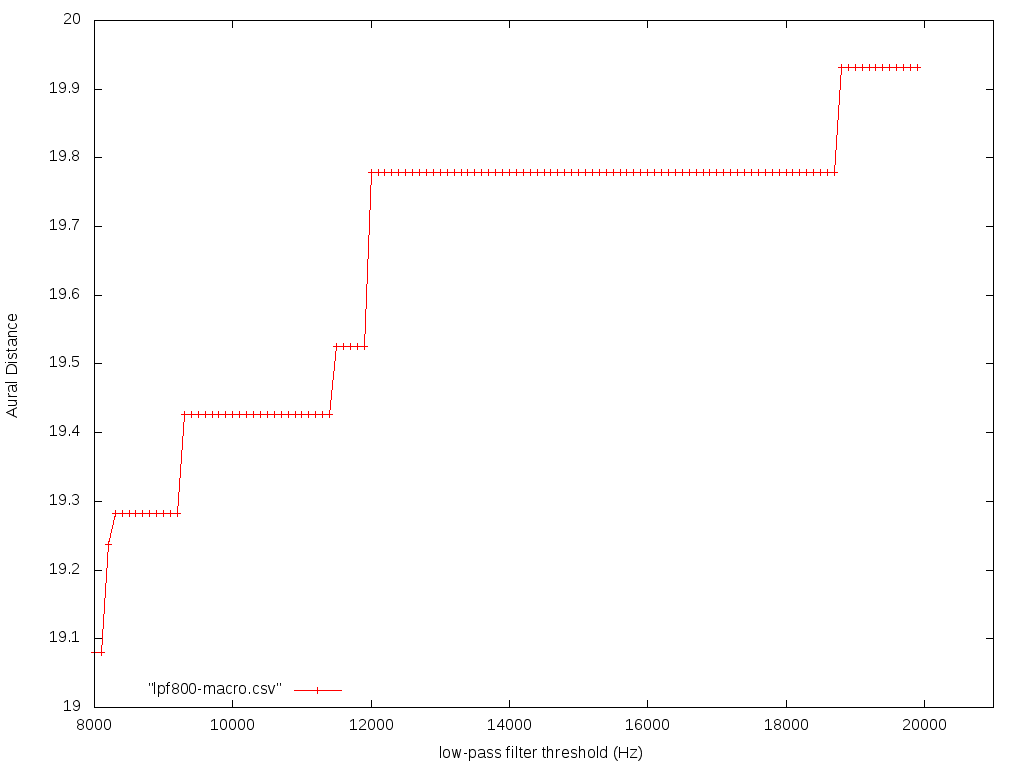
\includegraphics[width=\columnwidth]{figs/distCurveMacro} 
\begin{tikzpicture}[gnuplot]
%% generated with GNUPLOT 5.0p3 (Lua 5.1; terminal rev. 99, script rev. 100)
%% Sun 05 Aug 2018 11:53:28 PM EDT
\path (0.000,0.000) rectangle (8.890,8.890);
\gpcolor{color=gp lt color border}
\gpsetlinetype{gp lt border}
\gpsetlinewidth{1.00}
\draw[gp path] (1.504,0.985)--(1.684,0.985);
\draw[gp path] (8.337,0.985)--(8.157,0.985);
\node[gp node right] at (1.320,0.985) {$19$};
\draw[gp path] (1.504,1.739)--(1.684,1.739);
\draw[gp path] (8.337,1.739)--(8.157,1.739);
\node[gp node right] at (1.320,1.739) {$19.1$};
\draw[gp path] (1.504,2.492)--(1.684,2.492);
\draw[gp path] (8.337,2.492)--(8.157,2.492);
\node[gp node right] at (1.320,2.492) {$19.2$};
\draw[gp path] (1.504,3.246)--(1.684,3.246);
\draw[gp path] (8.337,3.246)--(8.157,3.246);
\node[gp node right] at (1.320,3.246) {$19.3$};
\draw[gp path] (1.504,3.999)--(1.684,3.999);
\draw[gp path] (8.337,3.999)--(8.157,3.999);
\node[gp node right] at (1.320,3.999) {$19.4$};
\draw[gp path] (1.504,4.753)--(1.684,4.753);
\draw[gp path] (8.337,4.753)--(8.157,4.753);
\node[gp node right] at (1.320,4.753) {$19.5$};
\draw[gp path] (1.504,5.507)--(1.684,5.507);
\draw[gp path] (8.337,5.507)--(8.157,5.507);
\node[gp node right] at (1.320,5.507) {$19.6$};
\draw[gp path] (1.504,6.260)--(1.684,6.260);
\draw[gp path] (8.337,6.260)--(8.157,6.260);
\node[gp node right] at (1.320,6.260) {$19.7$};
\draw[gp path] (1.504,7.014)--(1.684,7.014);
\draw[gp path] (8.337,7.014)--(8.157,7.014);
\node[gp node right] at (1.320,7.014) {$19.8$};
\draw[gp path] (1.504,7.767)--(1.684,7.767);
\draw[gp path] (8.337,7.767)--(8.157,7.767);
\node[gp node right] at (1.320,7.767) {$19.9$};
\draw[gp path] (1.504,8.521)--(1.684,8.521);
\draw[gp path] (8.337,8.521)--(8.157,8.521);
\node[gp node right] at (1.320,8.521) {$20$};
\draw[gp path] (1.504,0.985)--(1.504,1.165);
\draw[gp path] (1.504,8.521)--(1.504,8.341);
\node[gp node center] at (1.504,0.677) {$8000$};
\draw[gp path] (2.555,0.985)--(2.555,1.165);
\draw[gp path] (2.555,8.521)--(2.555,8.341);
\node[gp node center] at (2.555,0.677) {$10000$};
\draw[gp path] (3.606,0.985)--(3.606,1.165);
\draw[gp path] (3.606,8.521)--(3.606,8.341);
\node[gp node center] at (3.606,0.677) {$12000$};
\draw[gp path] (4.658,0.985)--(4.658,1.165);
\draw[gp path] (4.658,8.521)--(4.658,8.341);
\node[gp node center] at (4.658,0.677) {$14000$};
\draw[gp path] (5.709,0.985)--(5.709,1.165);
\draw[gp path] (5.709,8.521)--(5.709,8.341);
\node[gp node center] at (5.709,0.677) {$16000$};
\draw[gp path] (6.760,0.985)--(6.760,1.165);
\draw[gp path] (6.760,8.521)--(6.760,8.341);
\node[gp node center] at (6.760,0.677) {$18000$};
\draw[gp path] (7.811,0.985)--(7.811,1.165);
\draw[gp path] (7.811,8.521)--(7.811,8.341);
\node[gp node center] at (7.811,0.677) {$20000$};
\draw[gp path] (1.504,8.521)--(1.504,0.985)--(8.337,0.985)--(8.337,8.521)--cycle;
\node[gp node center,rotate=-270] at (0.246,4.753) {Aural Distance};
\node[gp node center] at (4.920,0.215) {low-pass filter threshold (Hz)};
\node[gp node right] at (5.000,1.319) {$\synthFilter = lpf(800)$};
\gpcolor{rgb color={0.580,0.000,0.827}}
\draw[gp path] (5.184,1.319)--(6.100,1.319);
\draw[gp path] (1.504,1.591)--(1.557,1.591)--(1.609,2.777)--(1.662,3.117)--(1.714,3.117)%
  --(1.767,3.117)--(1.819,3.117)--(1.872,3.117)--(1.924,3.117)--(1.977,3.117)--(2.030,3.117)%
  --(2.082,3.117)--(2.135,3.117)--(2.187,4.198)--(2.240,4.198)--(2.292,4.198)--(2.345,4.198)%
  --(2.398,4.198)--(2.450,4.198)--(2.503,4.198)--(2.555,4.198)--(2.608,4.198)--(2.660,4.198)%
  --(2.713,4.198)--(2.765,4.198)--(2.818,4.198)--(2.871,4.198)--(2.923,4.198)--(2.976,4.198)%
  --(3.028,4.198)--(3.081,4.198)--(3.133,4.198)--(3.186,4.198)--(3.239,4.198)--(3.291,4.198)%
  --(3.344,4.949)--(3.396,4.949)--(3.449,4.949)--(3.501,4.949)--(3.554,4.949)--(3.606,6.851)%
  --(3.659,6.851)--(3.712,6.851)--(3.764,6.851)--(3.817,6.851)--(3.869,6.851)--(3.922,6.851)%
  --(3.974,6.851)--(4.027,6.851)--(4.080,6.851)--(4.132,6.851)--(4.185,6.851)--(4.237,6.851)%
  --(4.290,6.851)--(4.342,6.851)--(4.395,6.851)--(4.447,6.851)--(4.500,6.851)--(4.553,6.851)%
  --(4.605,6.851)--(4.658,6.851)--(4.710,6.851)--(4.763,6.851)--(4.815,6.851)--(4.868,6.851)%
  --(4.921,6.851)--(4.973,6.851)--(5.026,6.851)--(5.078,6.851)--(5.131,6.851)--(5.183,6.851)%
  --(5.236,6.851)--(5.288,6.851)--(5.341,6.851)--(5.394,6.851)--(5.446,6.851)--(5.499,6.851)%
  --(5.551,6.851)--(5.604,6.851)--(5.656,6.851)--(5.709,6.851)--(5.761,6.851)--(5.814,6.851)%
  --(5.867,6.851)--(5.919,6.851)--(5.972,6.851)--(6.024,6.851)--(6.077,6.851)--(6.129,6.851)%
  --(6.182,6.851)--(6.235,6.851)--(6.287,6.851)--(6.340,6.851)--(6.392,6.851)--(6.445,6.851)%
  --(6.497,6.851)--(6.550,6.851)--(6.602,6.851)--(6.655,6.851)--(6.708,6.851)--(6.760,6.851)%
  --(6.813,6.851)--(6.865,6.851)--(6.918,6.851)--(6.970,6.851)--(7.023,6.851)--(7.076,6.851)%
  --(7.128,6.851)--(7.181,8.007)--(7.233,8.007)--(7.286,8.007)--(7.338,8.007)--(7.391,8.007)%
  --(7.443,8.007)--(7.496,8.007)--(7.549,8.007)--(7.601,8.007)--(7.654,8.007)--(7.706,8.007)%
  --(7.759,8.007);
\gpsetpointsize{4.00}
\gppoint{gp mark 1}{(1.504,1.591)}
\gppoint{gp mark 1}{(1.557,1.591)}
\gppoint{gp mark 1}{(1.609,2.777)}
\gppoint{gp mark 1}{(1.662,3.117)}
\gppoint{gp mark 1}{(1.714,3.117)}
\gppoint{gp mark 1}{(1.767,3.117)}
\gppoint{gp mark 1}{(1.819,3.117)}
\gppoint{gp mark 1}{(1.872,3.117)}
\gppoint{gp mark 1}{(1.924,3.117)}
\gppoint{gp mark 1}{(1.977,3.117)}
\gppoint{gp mark 1}{(2.030,3.117)}
\gppoint{gp mark 1}{(2.082,3.117)}
\gppoint{gp mark 1}{(2.135,3.117)}
\gppoint{gp mark 1}{(2.187,4.198)}
\gppoint{gp mark 1}{(2.240,4.198)}
\gppoint{gp mark 1}{(2.292,4.198)}
\gppoint{gp mark 1}{(2.345,4.198)}
\gppoint{gp mark 1}{(2.398,4.198)}
\gppoint{gp mark 1}{(2.450,4.198)}
\gppoint{gp mark 1}{(2.503,4.198)}
\gppoint{gp mark 1}{(2.555,4.198)}
\gppoint{gp mark 1}{(2.608,4.198)}
\gppoint{gp mark 1}{(2.660,4.198)}
\gppoint{gp mark 1}{(2.713,4.198)}
\gppoint{gp mark 1}{(2.765,4.198)}
\gppoint{gp mark 1}{(2.818,4.198)}
\gppoint{gp mark 1}{(2.871,4.198)}
\gppoint{gp mark 1}{(2.923,4.198)}
\gppoint{gp mark 1}{(2.976,4.198)}
\gppoint{gp mark 1}{(3.028,4.198)}
\gppoint{gp mark 1}{(3.081,4.198)}
\gppoint{gp mark 1}{(3.133,4.198)}
\gppoint{gp mark 1}{(3.186,4.198)}
\gppoint{gp mark 1}{(3.239,4.198)}
\gppoint{gp mark 1}{(3.291,4.198)}
\gppoint{gp mark 1}{(3.344,4.949)}
\gppoint{gp mark 1}{(3.396,4.949)}
\gppoint{gp mark 1}{(3.449,4.949)}
\gppoint{gp mark 1}{(3.501,4.949)}
\gppoint{gp mark 1}{(3.554,4.949)}
\gppoint{gp mark 1}{(3.606,6.851)}
\gppoint{gp mark 1}{(3.659,6.851)}
\gppoint{gp mark 1}{(3.712,6.851)}
\gppoint{gp mark 1}{(3.764,6.851)}
\gppoint{gp mark 1}{(3.817,6.851)}
\gppoint{gp mark 1}{(3.869,6.851)}
\gppoint{gp mark 1}{(3.922,6.851)}
\gppoint{gp mark 1}{(3.974,6.851)}
\gppoint{gp mark 1}{(4.027,6.851)}
\gppoint{gp mark 1}{(4.080,6.851)}
\gppoint{gp mark 1}{(4.132,6.851)}
\gppoint{gp mark 1}{(4.185,6.851)}
\gppoint{gp mark 1}{(4.237,6.851)}
\gppoint{gp mark 1}{(4.290,6.851)}
\gppoint{gp mark 1}{(4.342,6.851)}
\gppoint{gp mark 1}{(4.395,6.851)}
\gppoint{gp mark 1}{(4.447,6.851)}
\gppoint{gp mark 1}{(4.500,6.851)}
\gppoint{gp mark 1}{(4.553,6.851)}
\gppoint{gp mark 1}{(4.605,6.851)}
\gppoint{gp mark 1}{(4.658,6.851)}
\gppoint{gp mark 1}{(4.710,6.851)}
\gppoint{gp mark 1}{(4.763,6.851)}
\gppoint{gp mark 1}{(4.815,6.851)}
\gppoint{gp mark 1}{(4.868,6.851)}
\gppoint{gp mark 1}{(4.921,6.851)}
\gppoint{gp mark 1}{(4.973,6.851)}
\gppoint{gp mark 1}{(5.026,6.851)}
\gppoint{gp mark 1}{(5.078,6.851)}
\gppoint{gp mark 1}{(5.131,6.851)}
\gppoint{gp mark 1}{(5.183,6.851)}
\gppoint{gp mark 1}{(5.236,6.851)}
\gppoint{gp mark 1}{(5.288,6.851)}
\gppoint{gp mark 1}{(5.341,6.851)}
\gppoint{gp mark 1}{(5.394,6.851)}
\gppoint{gp mark 1}{(5.446,6.851)}
\gppoint{gp mark 1}{(5.499,6.851)}
\gppoint{gp mark 1}{(5.551,6.851)}
\gppoint{gp mark 1}{(5.604,6.851)}
\gppoint{gp mark 1}{(5.656,6.851)}
\gppoint{gp mark 1}{(5.709,6.851)}
\gppoint{gp mark 1}{(5.761,6.851)}
\gppoint{gp mark 1}{(5.814,6.851)}
\gppoint{gp mark 1}{(5.867,6.851)}
\gppoint{gp mark 1}{(5.919,6.851)}
\gppoint{gp mark 1}{(5.972,6.851)}
\gppoint{gp mark 1}{(6.024,6.851)}
\gppoint{gp mark 1}{(6.077,6.851)}
\gppoint{gp mark 1}{(6.129,6.851)}
\gppoint{gp mark 1}{(6.182,6.851)}
\gppoint{gp mark 1}{(6.235,6.851)}
\gppoint{gp mark 1}{(6.287,6.851)}
\gppoint{gp mark 1}{(6.340,6.851)}
\gppoint{gp mark 1}{(6.392,6.851)}
\gppoint{gp mark 1}{(6.445,6.851)}
\gppoint{gp mark 1}{(6.497,6.851)}
\gppoint{gp mark 1}{(6.550,6.851)}
\gppoint{gp mark 1}{(6.602,6.851)}
\gppoint{gp mark 1}{(6.655,6.851)}
\gppoint{gp mark 1}{(6.708,6.851)}
\gppoint{gp mark 1}{(6.760,6.851)}
\gppoint{gp mark 1}{(6.813,6.851)}
\gppoint{gp mark 1}{(6.865,6.851)}
\gppoint{gp mark 1}{(6.918,6.851)}
\gppoint{gp mark 1}{(6.970,6.851)}
\gppoint{gp mark 1}{(7.023,6.851)}
\gppoint{gp mark 1}{(7.076,6.851)}
\gppoint{gp mark 1}{(7.128,6.851)}
\gppoint{gp mark 1}{(7.181,8.007)}
\gppoint{gp mark 1}{(7.233,8.007)}
\gppoint{gp mark 1}{(7.286,8.007)}
\gppoint{gp mark 1}{(7.338,8.007)}
\gppoint{gp mark 1}{(7.391,8.007)}
\gppoint{gp mark 1}{(7.443,8.007)}
\gppoint{gp mark 1}{(7.496,8.007)}
\gppoint{gp mark 1}{(7.549,8.007)}
\gppoint{gp mark 1}{(7.601,8.007)}
\gppoint{gp mark 1}{(7.654,8.007)}
\gppoint{gp mark 1}{(7.706,8.007)}
\gppoint{gp mark 1}{(7.759,8.007)}
\gppoint{gp mark 1}{(5.642,1.319)}
\gpcolor{color=gp lt color border}
\draw[gp path] (1.504,8.521)--(1.504,0.985)--(8.337,0.985)--(8.337,8.521)--cycle;
%% coordinates of the plot area
\gpdefrectangularnode{gp plot 1}{\pgfpoint{1.504cm}{0.985cm}}{\pgfpoint{8.337cm}{8.521cm}}
\end{tikzpicture}
%% gnuplot variables

\caption{Looking at the portion of a curve from Figure~\ref{fig:distCurves} between 8k Hz and 20k Hz, we see the aural distance function is not perfectly convex on the macro scale. In this case, that is because the sample has very few frequencies above the 8k Hz range.}
\label{fig:macroDist}
\end{figure}

On the macro scale, we face the challenge that the distance function is again not convex -- there are many local minima and long plateaus, as shown in Figure~\ref{fig:macroDist}.
In order to overcome this, we must carefully pick the initial value for gradient descent.
If we pick a value in the middle of a plateau, the gradient descent algorithm will not find any significant gradient, and conclude we have reached the convergence condition.
In our current implementation, we iterate at large intervals (1000 Hz) of possible threshold values for both low and high pass filters.
We choose possible DSP programs that use only low pass, only high pass, and both low and high pass filters.
After evaluating these, we take the lowest cost initial DSP program, and start gradient descent from that point.

Finally, one of the key parts of a good application of gradient descent is the choice of the parameters such as the learning rate and the convergence goal.
These parameters must be adjusted based on the values observed from the cost (in our case, distance) function.
While the details of tuning gradient descent are outside the scope of this paper, it suffices to note that any change in the distance metric will likely also require a readjustment of these parameters.

